\PassOptionsToPackage{unicode=true}{hyperref} % options for packages loaded elsewhere
\PassOptionsToPackage{hyphens}{url}
%
\documentclass[]{article}
\usepackage{lmodern}
\usepackage{amssymb,amsmath}
\usepackage{ifxetex,ifluatex}
\usepackage{fixltx2e} % provides \textsubscript
\ifnum 0\ifxetex 1\fi\ifluatex 1\fi=0 % if pdftex
  \usepackage[T1]{fontenc}
  \usepackage[utf8]{inputenc}
  \usepackage{textcomp} % provides euro and other symbols
\else % if luatex or xelatex
  \usepackage{unicode-math}
  \defaultfontfeatures{Ligatures=TeX,Scale=MatchLowercase}
\fi
% use upquote if available, for straight quotes in verbatim environments
\IfFileExists{upquote.sty}{\usepackage{upquote}}{}
% use microtype if available
\IfFileExists{microtype.sty}{%
\usepackage[]{microtype}
\UseMicrotypeSet[protrusion]{basicmath} % disable protrusion for tt fonts
}{}
\IfFileExists{parskip.sty}{%
\usepackage{parskip}
}{% else
\setlength{\parindent}{0pt}
\setlength{\parskip}{6pt plus 2pt minus 1pt}
}
\usepackage{hyperref}
\hypersetup{
            pdfborder={0 0 0},
            breaklinks=true}
\urlstyle{same}  % don't use monospace font for urls
\usepackage[margin=1in]{geometry}
\usepackage{color}
\usepackage{fancyvrb}
\newcommand{\VerbBar}{|}
\newcommand{\VERB}{\Verb[commandchars=\\\{\}]}
\DefineVerbatimEnvironment{Highlighting}{Verbatim}{commandchars=\\\{\}}
% Add ',fontsize=\small' for more characters per line
\usepackage{framed}
\definecolor{shadecolor}{RGB}{248,248,248}
\newenvironment{Shaded}{\begin{snugshade}}{\end{snugshade}}
\newcommand{\AlertTok}[1]{\textcolor[rgb]{0.94,0.16,0.16}{#1}}
\newcommand{\AnnotationTok}[1]{\textcolor[rgb]{0.56,0.35,0.01}{\textbf{\textit{#1}}}}
\newcommand{\AttributeTok}[1]{\textcolor[rgb]{0.77,0.63,0.00}{#1}}
\newcommand{\BaseNTok}[1]{\textcolor[rgb]{0.00,0.00,0.81}{#1}}
\newcommand{\BuiltInTok}[1]{#1}
\newcommand{\CharTok}[1]{\textcolor[rgb]{0.31,0.60,0.02}{#1}}
\newcommand{\CommentTok}[1]{\textcolor[rgb]{0.56,0.35,0.01}{\textit{#1}}}
\newcommand{\CommentVarTok}[1]{\textcolor[rgb]{0.56,0.35,0.01}{\textbf{\textit{#1}}}}
\newcommand{\ConstantTok}[1]{\textcolor[rgb]{0.00,0.00,0.00}{#1}}
\newcommand{\ControlFlowTok}[1]{\textcolor[rgb]{0.13,0.29,0.53}{\textbf{#1}}}
\newcommand{\DataTypeTok}[1]{\textcolor[rgb]{0.13,0.29,0.53}{#1}}
\newcommand{\DecValTok}[1]{\textcolor[rgb]{0.00,0.00,0.81}{#1}}
\newcommand{\DocumentationTok}[1]{\textcolor[rgb]{0.56,0.35,0.01}{\textbf{\textit{#1}}}}
\newcommand{\ErrorTok}[1]{\textcolor[rgb]{0.64,0.00,0.00}{\textbf{#1}}}
\newcommand{\ExtensionTok}[1]{#1}
\newcommand{\FloatTok}[1]{\textcolor[rgb]{0.00,0.00,0.81}{#1}}
\newcommand{\FunctionTok}[1]{\textcolor[rgb]{0.00,0.00,0.00}{#1}}
\newcommand{\ImportTok}[1]{#1}
\newcommand{\InformationTok}[1]{\textcolor[rgb]{0.56,0.35,0.01}{\textbf{\textit{#1}}}}
\newcommand{\KeywordTok}[1]{\textcolor[rgb]{0.13,0.29,0.53}{\textbf{#1}}}
\newcommand{\NormalTok}[1]{#1}
\newcommand{\OperatorTok}[1]{\textcolor[rgb]{0.81,0.36,0.00}{\textbf{#1}}}
\newcommand{\OtherTok}[1]{\textcolor[rgb]{0.56,0.35,0.01}{#1}}
\newcommand{\PreprocessorTok}[1]{\textcolor[rgb]{0.56,0.35,0.01}{\textit{#1}}}
\newcommand{\RegionMarkerTok}[1]{#1}
\newcommand{\SpecialCharTok}[1]{\textcolor[rgb]{0.00,0.00,0.00}{#1}}
\newcommand{\SpecialStringTok}[1]{\textcolor[rgb]{0.31,0.60,0.02}{#1}}
\newcommand{\StringTok}[1]{\textcolor[rgb]{0.31,0.60,0.02}{#1}}
\newcommand{\VariableTok}[1]{\textcolor[rgb]{0.00,0.00,0.00}{#1}}
\newcommand{\VerbatimStringTok}[1]{\textcolor[rgb]{0.31,0.60,0.02}{#1}}
\newcommand{\WarningTok}[1]{\textcolor[rgb]{0.56,0.35,0.01}{\textbf{\textit{#1}}}}
\usepackage{graphicx,grffile}
\makeatletter
\def\maxwidth{\ifdim\Gin@nat@width>\linewidth\linewidth\else\Gin@nat@width\fi}
\def\maxheight{\ifdim\Gin@nat@height>\textheight\textheight\else\Gin@nat@height\fi}
\makeatother
% Scale images if necessary, so that they will not overflow the page
% margins by default, and it is still possible to overwrite the defaults
% using explicit options in \includegraphics[width, height, ...]{}
\setkeys{Gin}{width=\maxwidth,height=\maxheight,keepaspectratio}
\setlength{\emergencystretch}{3em}  % prevent overfull lines
\providecommand{\tightlist}{%
  \setlength{\itemsep}{0pt}\setlength{\parskip}{0pt}}
\setcounter{secnumdepth}{0}
% Redefines (sub)paragraphs to behave more like sections
\ifx\paragraph\undefined\else
\let\oldparagraph\paragraph
\renewcommand{\paragraph}[1]{\oldparagraph{#1}\mbox{}}
\fi
\ifx\subparagraph\undefined\else
\let\oldsubparagraph\subparagraph
\renewcommand{\subparagraph}[1]{\oldsubparagraph{#1}\mbox{}}
\fi

% set default figure placement to htbp
\makeatletter
\def\fps@figure{htbp}
\makeatother

\usepackage{stmaryrd}
\usepackage{amsfonts}
\usepackage{amsmath}

\author{}
\date{\vspace{-2.5em}}

\begin{document}

\begin{titlepage}
\newcommand{\HRule}{\rule{\linewidth}{0.5mm}}
\center
\textsc{\LARGE
STA212 - Méthodes de rééchantillonnage} \\[2cm]
\LARGE Enseignant: Mohammed Sedki  \\[2cm]

\HRule \\[0.4cm]
{ \huge \bfseries Devoir : aspects pratiques \\[0.15cm] }
\HRule \\[3cm] \LARGE
Romin DURAND \\
Loukman Eltarr
\\[3cm]
\today \\ [1cm]
\end{titlepage}

\hypertarget{arbre-de-duxe9cision-unique}{%
\section{Arbre de décision unique}\label{arbre-de-duxe9cision-unique}}

\begin{Shaded}
\begin{Highlighting}[]
\KeywordTok{setwd}\NormalTok{(}\StringTok{'~/Cours/STA212/STA212DM'}\NormalTok{)}
\CommentTok{#setwd("/home/lokmen/Documents/ENSTA/STAT/STA212/STA212DM")}
\KeywordTok{rm}\NormalTok{(}\DataTypeTok{list =} \KeywordTok{objects}\NormalTok{())}
\KeywordTok{graphics.off}\NormalTok{()}
\NormalTok{OJ=}\KeywordTok{read.csv}\NormalTok{(}\StringTok{"oj.csv"}\NormalTok{, }\DataTypeTok{header =} \OtherTok{TRUE}\NormalTok{)}
\CommentTok{#View(OJ)}
\end{Highlighting}
\end{Shaded}

On regarde la nature de nos données. On a 1070 observations pour 18
variables différentes. Les variables categorielles sont
\(\texttt{Purchase}\) qui admet deux niveaux, et \(\texttt{Store 7}\)
qui admet aussi deux niveaux. Les autres sont numériques.

\begin{Shaded}
\begin{Highlighting}[]
\KeywordTok{str}\NormalTok{(OJ) }
\end{Highlighting}
\end{Shaded}

\begin{verbatim}
## 'data.frame':    1070 obs. of  18 variables:
##  $ Purchase      : Factor w/ 2 levels "CH","MM": 1 1 1 2 1 1 1 1 1 1 ...
##  $ WeekofPurchase: int  237 239 245 227 228 230 232 234 235 238 ...
##  $ StoreID       : int  1 1 1 1 7 7 7 7 7 7 ...
##  $ PriceCH       : num  1.75 1.75 1.86 1.69 1.69 1.69 1.69 1.75 1.75 1.75 ...
##  $ PriceMM       : num  1.99 1.99 2.09 1.69 1.69 1.99 1.99 1.99 1.99 1.99 ...
##  $ DiscCH        : num  0 0 0.17 0 0 0 0 0 0 0 ...
##  $ DiscMM        : num  0 0.3 0 0 0 0 0.4 0.4 0.4 0.4 ...
##  $ SpecialCH     : int  0 0 0 0 0 0 1 1 0 0 ...
##  $ SpecialMM     : int  0 1 0 0 0 1 1 0 0 0 ...
##  $ LoyalCH       : num  0.5 0.6 0.68 0.4 0.957 ...
##  $ SalePriceMM   : num  1.99 1.69 2.09 1.69 1.69 1.99 1.59 1.59 1.59 1.59 ...
##  $ SalePriceCH   : num  1.75 1.75 1.69 1.69 1.69 1.69 1.69 1.75 1.75 1.75 ...
##  $ PriceDiff     : num  0.24 -0.06 0.4 0 0 0.3 -0.1 -0.16 -0.16 -0.16 ...
##  $ Store7        : Factor w/ 2 levels "No","Yes": 1 1 1 1 2 2 2 2 2 2 ...
##  $ PctDiscMM     : num  0 0.151 0 0 0 ...
##  $ PctDiscCH     : num  0 0 0.0914 0 0 ...
##  $ ListPriceDiff : num  0.24 0.24 0.23 0 0 0.3 0.3 0.24 0.24 0.24 ...
##  $ STORE         : int  1 1 1 1 0 0 0 0 0 0 ...
\end{verbatim}

\hypertarget{analyse-univariuxe9e}{%
\subsection{Analyse Univariée}\label{analyse-univariuxe9e}}

On procéde à une analyse univariée des variables. On se sert de la
description des variables ainsi que des commandes \(\texttt{summary}\),
\(\texttt{plot}\) et \(\texttt{table}\).

Par exemple, on peut voir que les variables \(\texttt{SpecialCH}\) et
\(\texttt{SpecialMM}\) prennent seulement les valeurs 0 et 1.

\begin{Shaded}
\begin{Highlighting}[]
\KeywordTok{table}\NormalTok{(OJ}\OperatorTok{$}\NormalTok{SpecialCH)}
\end{Highlighting}
\end{Shaded}

\begin{verbatim}
## 
##   0   1 
## 912 158
\end{verbatim}

\begin{Shaded}
\begin{Highlighting}[]
\KeywordTok{plot}\NormalTok{(OJ}\OperatorTok{$}\NormalTok{SpecialCH)}
\end{Highlighting}
\end{Shaded}

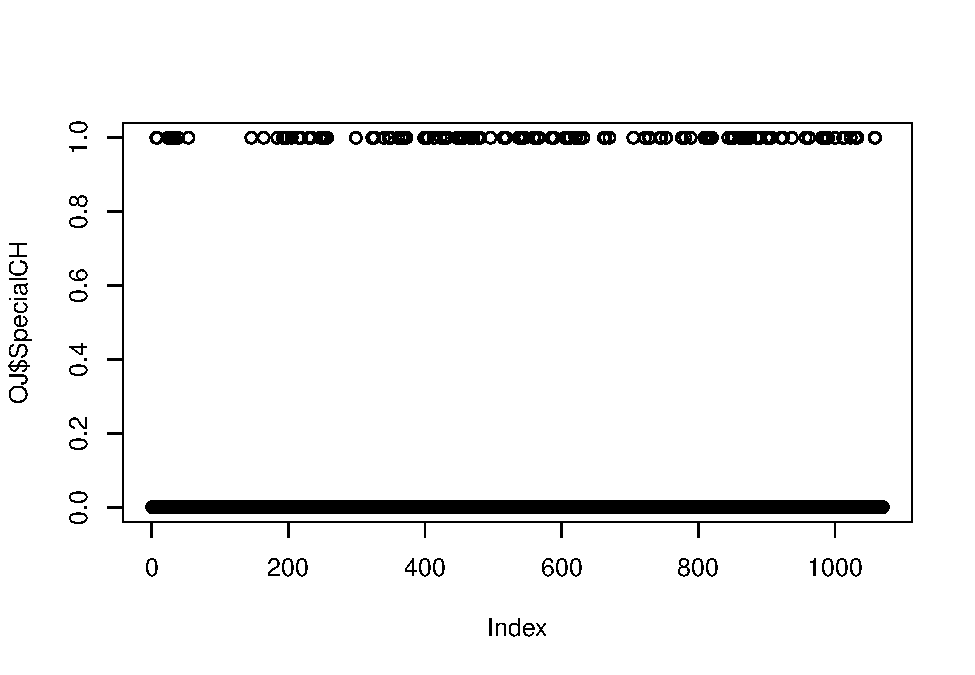
\includegraphics{durand_eltarr_files/figure-latex/unnamed-chunk-3-1.pdf}

\begin{Shaded}
\begin{Highlighting}[]
\KeywordTok{table}\NormalTok{(OJ}\OperatorTok{$}\NormalTok{SpecialMM)}
\end{Highlighting}
\end{Shaded}

\begin{verbatim}
## 
##   0   1 
## 897 173
\end{verbatim}

\begin{Shaded}
\begin{Highlighting}[]
\KeywordTok{plot}\NormalTok{(OJ}\OperatorTok{$}\NormalTok{SpecialMM)}
\end{Highlighting}
\end{Shaded}

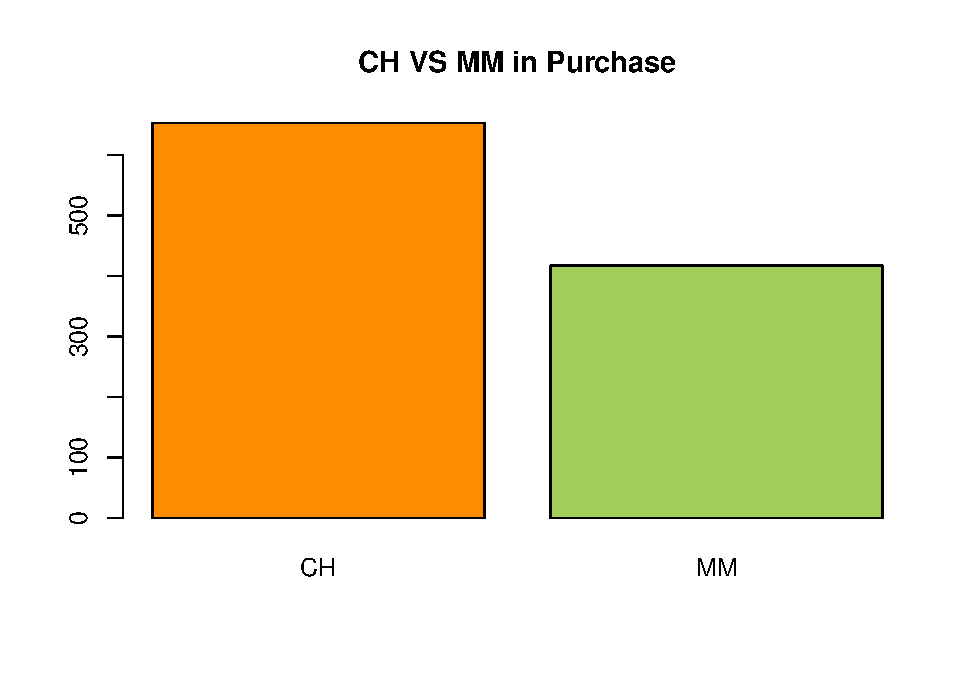
\includegraphics{durand_eltarr_files/figure-latex/unnamed-chunk-4-1.pdf}

De la même manière \(\texttt{STORE}\) ne prend que les valeurs entre 0
et 4.

\begin{Shaded}
\begin{Highlighting}[]
\KeywordTok{table}\NormalTok{(OJ}\OperatorTok{$}\NormalTok{STORE)}
\end{Highlighting}
\end{Shaded}

\begin{verbatim}
## 
##   0   1   2   3   4 
## 356 157 222 196 139
\end{verbatim}

\begin{Shaded}
\begin{Highlighting}[]
\KeywordTok{plot}\NormalTok{(OJ}\OperatorTok{$}\NormalTok{STORE)}
\end{Highlighting}
\end{Shaded}

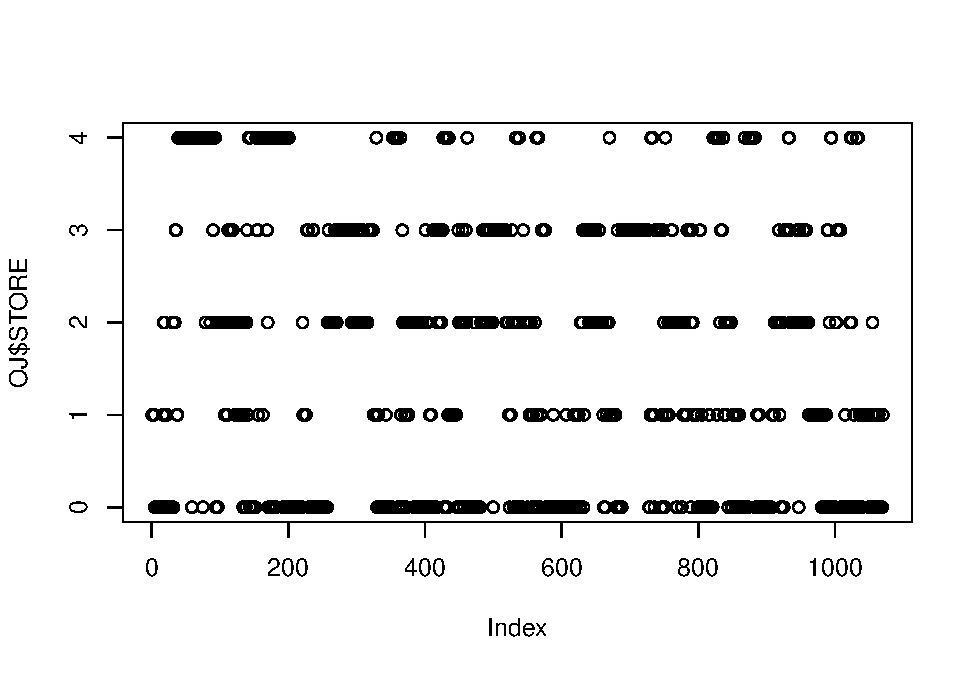
\includegraphics{durand_eltarr_files/figure-latex/unnamed-chunk-5-1.pdf}

On préfère alors les transformer en variables catégorielles:

\begin{Shaded}
\begin{Highlighting}[]
\NormalTok{OJ}\OperatorTok{$}\NormalTok{SpecialMM <-}\StringTok{ }\KeywordTok{as.factor}\NormalTok{(OJ}\OperatorTok{$}\NormalTok{SpecialMM)}
\NormalTok{OJ}\OperatorTok{$}\NormalTok{SpecialCH <-}\StringTok{ }\KeywordTok{as.factor}\NormalTok{(OJ}\OperatorTok{$}\NormalTok{SpecialCH)}
\NormalTok{OJ}\OperatorTok{$}\NormalTok{STORE <-}\StringTok{ }\KeywordTok{as.factor}\NormalTok{(OJ}\OperatorTok{$}\NormalTok{STORE}\OperatorTok{+}\DecValTok{1}\NormalTok{) }\CommentTok{## On préfère avoir des valeurs entre 1 et 5.}
\end{Highlighting}
\end{Shaded}

On regarde la proportion de ``MM'' par rapport à celle de ``CH''. Il ya
plus de CH que de MM qui ont été commendés. La proportion est de
61\%-39\%.

\begin{Shaded}
\begin{Highlighting}[]
\KeywordTok{table}\NormalTok{(OJ}\OperatorTok{$}\NormalTok{Purchase)}\OperatorTok{/}\KeywordTok{nrow}\NormalTok{(OJ)}
\end{Highlighting}
\end{Shaded}

\begin{verbatim}
## 
##        CH        MM 
## 0.6102804 0.3897196
\end{verbatim}

\begin{Shaded}
\begin{Highlighting}[]
\KeywordTok{plot}\NormalTok{(OJ}\OperatorTok{$}\NormalTok{Purchase, }\DataTypeTok{main =}\StringTok{"CH VS MM in Purchase"}\NormalTok{,}\DataTypeTok{col=}\KeywordTok{c}\NormalTok{(}\StringTok{"darkorange"}\NormalTok{,}\StringTok{"darkolivegreen3"}\NormalTok{))}
\end{Highlighting}
\end{Shaded}

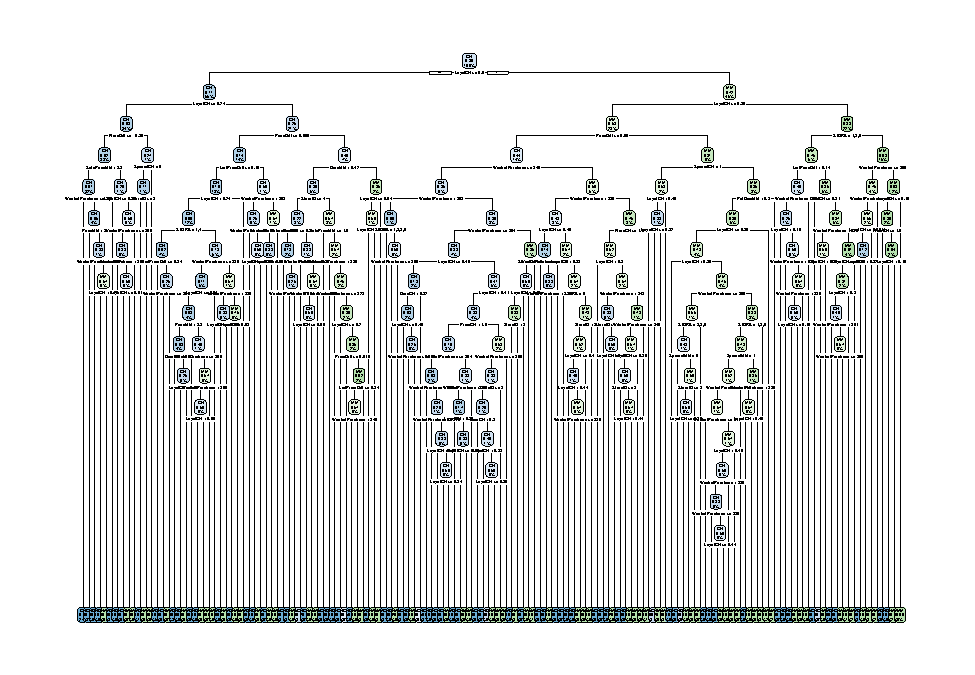
\includegraphics{durand_eltarr_files/figure-latex/unnamed-chunk-7-1.pdf}
\#\# Question 1 On divise d'abord notre jeu de donnée en une partie
\textbf{train} et une partie \textbf{test}

\begin{Shaded}
\begin{Highlighting}[]
\KeywordTok{set.seed}\NormalTok{(}\DecValTok{2}\NormalTok{) }\CommentTok{## On précise la graine afin d'avoir la reproductibilité}
\NormalTok{size_sample=}\DecValTok{800} \CommentTok{## tailer de notre echantillon train}
\NormalTok{train <-}\StringTok{ }\KeywordTok{sample}\NormalTok{(}\KeywordTok{c}\NormalTok{(}\DecValTok{1}\OperatorTok{:}\KeywordTok{nrow}\NormalTok{(OJ)), }\DataTypeTok{size=}\KeywordTok{floor}\NormalTok{(size_sample)) }\CommentTok{## list comportant l'index de la partie train}
\end{Highlighting}
\end{Shaded}

\hypertarget{question-2}{%
\subsection{Question 2}\label{question-2}}

On va utiliser l'apprentissage par arbre de décision pour faire un
prédction sur la partie test à partir de la partie train. On utilise
d'baord un arbre obtenu sans élagage puis un autre avec élagage, on
comparera ensuite la qualité des deux prédictions.

\begin{Shaded}
\begin{Highlighting}[]
\KeywordTok{require}\NormalTok{(rpart)}
\KeywordTok{require}\NormalTok{(rpart.plot)}
\end{Highlighting}
\end{Shaded}

\begin{verbatim}
## Warning: package 'rpart.plot' was built under R version 3.6.3
\end{verbatim}

\begin{Shaded}
\begin{Highlighting}[]
\CommentTok{## Arbre sans élagage}
\CommentTok{#   # Avec minsplit =1 on continue à explorer un noeau tant qu'il y a plus d'une seule variable }
\CommentTok{#   # cp = 0 indique qu'on explore un noeau même si il n'apporte pas de précision supplémentaire }
\CommentTok{#   # xval= 10 pour le nombre de fold dans notre validation croisée}
\NormalTok{three}\FloatTok{.0}\NormalTok{ <-}\StringTok{ }\KeywordTok{rpart}\NormalTok{(Purchase}\OperatorTok{~}\NormalTok{.,}
                \DataTypeTok{data=}\NormalTok{OJ[train,], }
                \DataTypeTok{control=}\KeywordTok{rpart.control}\NormalTok{(}\DataTypeTok{minsplit=}\DecValTok{1}\NormalTok{,}\DataTypeTok{cp=}\DecValTok{0}\NormalTok{, }\DataTypeTok{xval=}\DecValTok{10}\NormalTok{),}\DataTypeTok{model =}\OtherTok{TRUE}\NormalTok{)}
\KeywordTok{rpart.plot}\NormalTok{(three}\FloatTok{.0}\NormalTok{)}
\end{Highlighting}
\end{Shaded}

\begin{verbatim}
## Warning: labs do not fit even at cex 0.15, there may be some overplotting
\end{verbatim}

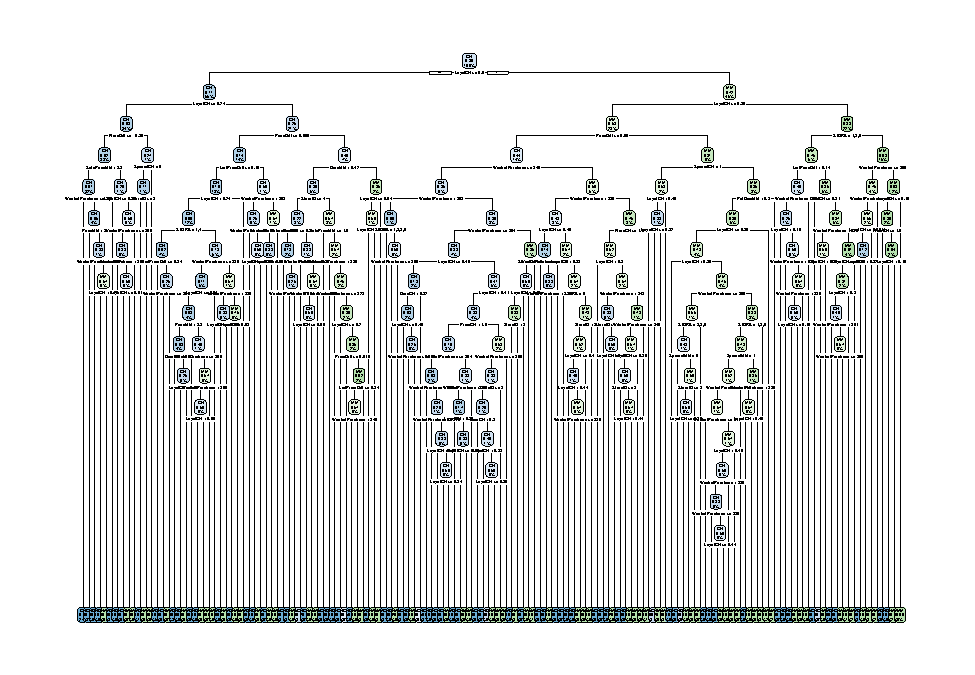
\includegraphics{durand_eltarr_files/figure-latex/unnamed-chunk-10-1.pdf}

\begin{Shaded}
\begin{Highlighting}[]
\CommentTok{## Arbre avec élagage}
\NormalTok{three}\FloatTok{.1}\NormalTok{ <-}\StringTok{ }\KeywordTok{prune}\NormalTok{(three}\FloatTok{.0}\NormalTok{, }\DataTypeTok{cp =}\NormalTok{ three}\FloatTok{.0}\OperatorTok{$}\NormalTok{cptable[}\KeywordTok{which.min}\NormalTok{(three}\FloatTok{.0}\OperatorTok{$}\NormalTok{cptable[,}\StringTok{"xerror"}\NormalTok{]),}\StringTok{"CP"}\NormalTok{],}\DataTypeTok{model =}\OtherTok{TRUE}\NormalTok{)}
\KeywordTok{rpart.plot}\NormalTok{(three}\FloatTok{.1}\NormalTok{)}
\end{Highlighting}
\end{Shaded}

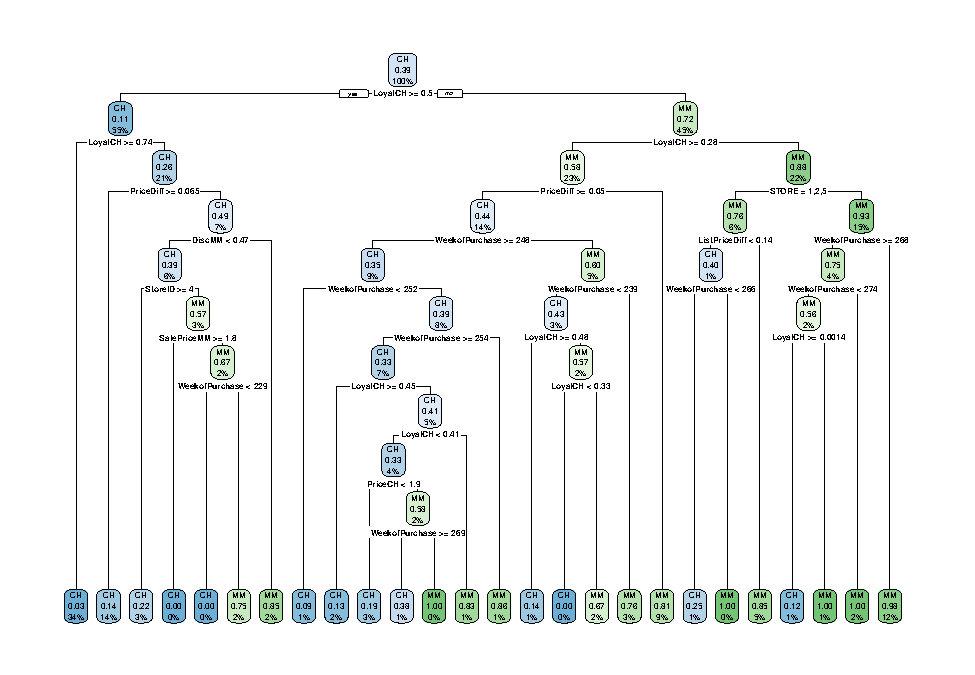
\includegraphics{durand_eltarr_files/figure-latex/unnamed-chunk-10-2.pdf}

On voit que le graphique obtenu sans élagage est difficilement lisible
ou interpretable. Il présente aussi probablement un problèmes
d'affichage au vu du de la trop importante information qu'il contient.
Au contraire, pour l'arbre pourlequel on a utilisé l'élagage, on voit
clairement les noeuds internees et les feuilles ainsi que les
proportions associées. \#\#\# Erreurs de Prédiction On compare ensuite
leurs erreurs de prediction.

\begin{Shaded}
\begin{Highlighting}[]
\NormalTok{pred}\FloatTok{.0}\NormalTok{ <-}\StringTok{ }\KeywordTok{predict}\NormalTok{(three}\FloatTok{.0}\NormalTok{, OJ, }\DataTypeTok{type=}\StringTok{"class"}\NormalTok{)}
\KeywordTok{mean}\NormalTok{(OJ}\OperatorTok{$}\NormalTok{Purchase[}\OperatorTok{-}\NormalTok{train]}\OperatorTok{!=}\NormalTok{pred}\FloatTok{.0}\NormalTok{[}\OperatorTok{-}\NormalTok{train])}
\end{Highlighting}
\end{Shaded}

\begin{verbatim}
## [1] 0.2222222
\end{verbatim}

\begin{Shaded}
\begin{Highlighting}[]
\NormalTok{pred}\FloatTok{.1}\NormalTok{ <-}\StringTok{ }\KeywordTok{predict}\NormalTok{(three}\FloatTok{.1}\NormalTok{, OJ, }\DataTypeTok{type=}\StringTok{"class"}\NormalTok{)}
\KeywordTok{mean}\NormalTok{(OJ}\OperatorTok{$}\NormalTok{Purchase[}\OperatorTok{-}\NormalTok{train]}\OperatorTok{!=}\NormalTok{pred}\FloatTok{.1}\NormalTok{[}\OperatorTok{-}\NormalTok{train])}
\end{Highlighting}
\end{Shaded}

\begin{verbatim}
## [1] 0.2259259
\end{verbatim}

On note que notre taux d'erreur est autour de 0.21 pour le premier
arbre. Ell est légerement inférieur à 0.16 pour le deuxième. Le second
est donc un légèrement meilleur.

\hypertarget{matrice-de-confusion}{%
\subsubsection{Matrice de Confusion}\label{matrice-de-confusion}}

On dresse alors une matrice de confusion. On a : * Pour l'abre sans
élagage : * 142 CH qui ont correctement été prédits. * 31 CH qui ont été
incorrectement prédits. * 26 MM qui ont été incorrectement prédits. * 71
MM qui ont correctement été prédits. Globalement la prediction est assez
bonne.

\begin{Shaded}
\begin{Highlighting}[]
\KeywordTok{table}\NormalTok{(OJ}\OperatorTok{$}\NormalTok{Purchase[}\OperatorTok{-}\NormalTok{train],pred}\FloatTok{.0}\NormalTok{[}\OperatorTok{-}\NormalTok{train],}\DataTypeTok{dnn =} \KeywordTok{c}\NormalTok{(}\StringTok{"Purchase"}\NormalTok{, }\StringTok{"Prediction"}\NormalTok{))}
\end{Highlighting}
\end{Shaded}

\begin{verbatim}
##         Prediction
## Purchase  CH  MM
##       CH 138  25
##       MM  35  72
\end{verbatim}

\begin{itemize}
\tightlist
\item
  Pour l'abre sans élagage :

  \begin{itemize}
  \tightlist
  \item
    151 CH qui ont correctement été prédits.
  \item
    22 CH qui ont été incorrectement prédits.
  \item
    21 MM qui ont été incorrectement prédits.
  \item
    77 MM qui ont correctement été prédits. Globalement la prediction
    est assez bonne.
  \end{itemize}
\end{itemize}

\begin{Shaded}
\begin{Highlighting}[]
\KeywordTok{table}\NormalTok{(OJ}\OperatorTok{$}\NormalTok{Purchase[}\OperatorTok{-}\NormalTok{train],pred}\FloatTok{.1}\NormalTok{[}\OperatorTok{-}\NormalTok{train],}\DataTypeTok{dnn =} \KeywordTok{c}\NormalTok{(}\StringTok{"Purchase"}\NormalTok{, }\StringTok{"Prediction"}\NormalTok{))}
\end{Highlighting}
\end{Shaded}

\begin{verbatim}
##         Prediction
## Purchase  CH  MM
##       CH 134  29
##       MM  32  75
\end{verbatim}

\hypertarget{question-3}{%
\subsection{Question 3}\label{question-3}}

\begin{Shaded}
\begin{Highlighting}[]
\KeywordTok{rpart.plot}\NormalTok{(three}\FloatTok{.1}\NormalTok{)}
\end{Highlighting}
\end{Shaded}

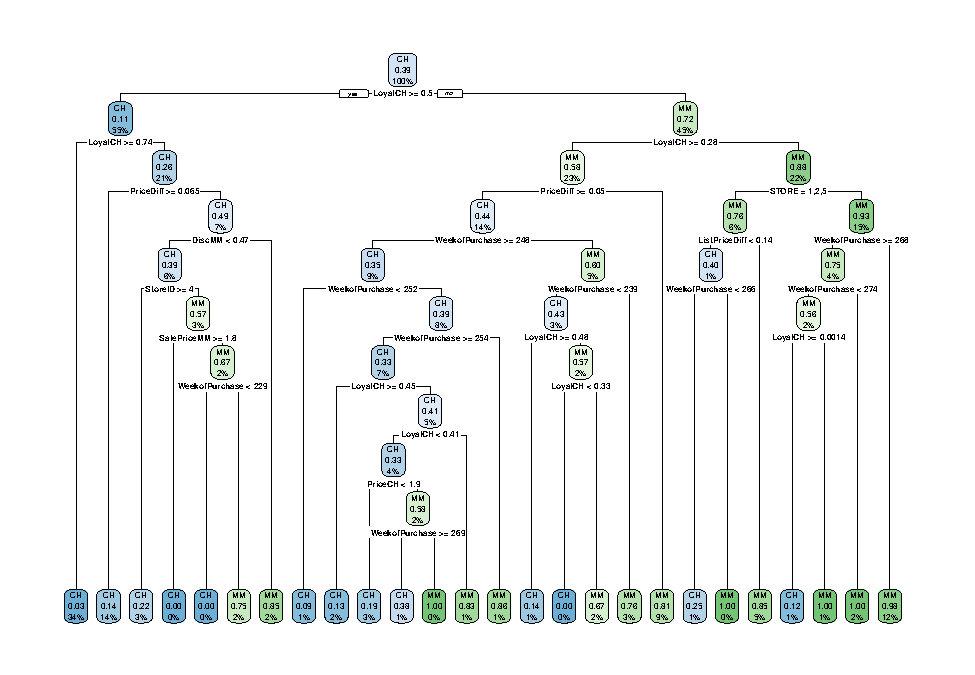
\includegraphics{durand_eltarr_files/figure-latex/unnamed-chunk-14-1.pdf}

On peut observer l'importance relative des variables.

\begin{Shaded}
\begin{Highlighting}[]
\NormalTok{three}\FloatTok{.1}\OperatorTok{$}\NormalTok{variable.importance}
\end{Highlighting}
\end{Shaded}

\begin{verbatim}
##        LoyalCH WeekofPurchase        StoreID          STORE        PriceMM 
##     188.526325      48.116729      41.142199      39.069757      31.727448 
##    SalePriceMM      PriceDiff        PriceCH         DiscMM      PctDiscMM 
##      31.264888      31.110619      24.459878      21.170419      20.986853 
##  ListPriceDiff    SalePriceCH         DiscCH      SpecialMM         Store7 
##      16.450657       7.363646       4.044643       3.730935       3.259171 
##      PctDiscCH 
##       3.062500
\end{verbatim}

\begin{Shaded}
\begin{Highlighting}[]
\KeywordTok{require}\NormalTok{(lattice)}
\KeywordTok{barchart}\NormalTok{(three}\FloatTok{.1}\OperatorTok{$}\NormalTok{variable.importance,}\DataTypeTok{xlab =} \StringTok{"Variables"}\NormalTok{, }\DataTypeTok{ylab =} \StringTok{"Importance"}\NormalTok{, }\DataTypeTok{main=}\StringTok{"Impotance des Variables"}\NormalTok{,}\DataTypeTok{col=}\KeywordTok{c}\NormalTok{(}\StringTok{'cornflowerblue'}\NormalTok{,}\StringTok{'chocolate3'}\NormalTok{,}\StringTok{'aquamarine2'}\NormalTok{,}\StringTok{'brown2'}\NormalTok{,}\StringTok{'burlywood3'}\NormalTok{,}\StringTok{'slategray2'}\NormalTok{,}\StringTok{'khaki4'}\NormalTok{,}\StringTok{'peru'}\NormalTok{,}\StringTok{'skyblue2'}\NormalTok{,}\StringTok{'violet'}\NormalTok{,}\StringTok{'darkorange1'}\NormalTok{,}\StringTok{'gold2'}\NormalTok{,}\StringTok{'lightpink4'}\NormalTok{,}\StringTok{'seagreen4'}\NormalTok{))}
\end{Highlighting}
\end{Shaded}

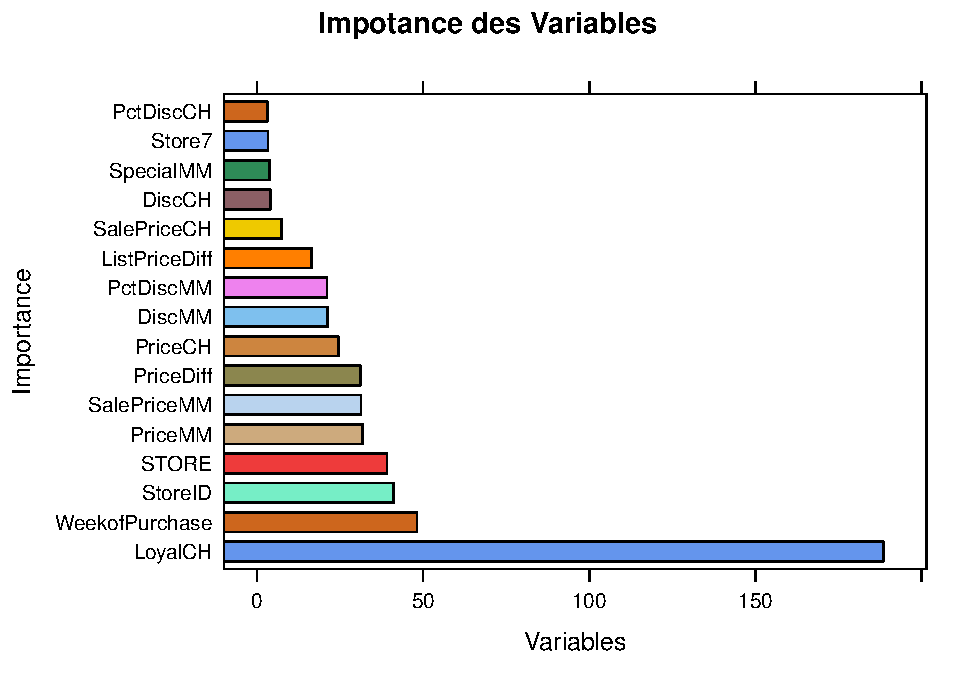
\includegraphics{durand_eltarr_files/figure-latex/unnamed-chunk-16-1.pdf}

\hypertarget{foruxeat-aluxe9atoires}{%
\section{Forêt aléatoires}\label{foruxeat-aluxe9atoires}}

Il faut tout d'abord changer la variable Class en variable factor :

\begin{Shaded}
\begin{Highlighting}[]
\NormalTok{email}\OperatorTok{$}\NormalTok{Class =}\StringTok{ }\KeywordTok{as.factor}\NormalTok{(email}\OperatorTok{$}\NormalTok{Class)}
\end{Highlighting}
\end{Shaded}

\hypertarget{question-4}{%
\subsection{Question 4}\label{question-4}}

\begin{Shaded}
\begin{Highlighting}[]
\KeywordTok{require}\NormalTok{(rpart)}
\KeywordTok{require}\NormalTok{(rpart.plot)}
\KeywordTok{require}\NormalTok{(ipred)}
\KeywordTok{require}\NormalTok{(caret)}
\KeywordTok{require}\NormalTok{(randomForest)}
\KeywordTok{require}\NormalTok{(doParallel)}
\end{Highlighting}
\end{Shaded}

\begin{Shaded}
\begin{Highlighting}[]
\NormalTok{N =}\StringTok{ }\KeywordTok{nrow}\NormalTok{(email)}
\KeywordTok{set.seed}\NormalTok{(}\DecValTok{103}\NormalTok{)}
\NormalTok{train =}\StringTok{ }\KeywordTok{sample}\NormalTok{(}\DecValTok{1}\OperatorTok{:}\NormalTok{N, }\KeywordTok{round}\NormalTok{(}\FloatTok{0.75}\OperatorTok{*}\NormalTok{N))}
\NormalTok{email.tr =}\StringTok{ }\NormalTok{email[train,]}
\NormalTok{email.te =}\StringTok{ }\NormalTok{email[}\OperatorTok{-}\NormalTok{train,]}
\end{Highlighting}
\end{Shaded}

Ajustons tout d'abord un arbre sans élagage :

\begin{Shaded}
\begin{Highlighting}[]
\NormalTok{cart}\FloatTok{.0}\NormalTok{ <-}\StringTok{ }\KeywordTok{rpart}\NormalTok{(Class}\OperatorTok{~}\NormalTok{.,}
                \DataTypeTok{data=}\NormalTok{email.tr, }
                \DataTypeTok{control=}\KeywordTok{rpart.control}\NormalTok{(}\DataTypeTok{minsplit=}\DecValTok{1}\NormalTok{,}\DataTypeTok{cp=}\DecValTok{0}\NormalTok{, }\DataTypeTok{xval=}\DecValTok{30}\NormalTok{)) }\CommentTok{# minsplit=1,cp=0}
                                                                \CommentTok{# pour avoir un arbre le}
                                                                \CommentTok{# plus profond possible}
\KeywordTok{rpart.plot}\NormalTok{(cart}\FloatTok{.0}\NormalTok{)}
\end{Highlighting}
\end{Shaded}

\begin{verbatim}
## Warning: labs do not fit even at cex 0.15, there may be some overplotting
\end{verbatim}

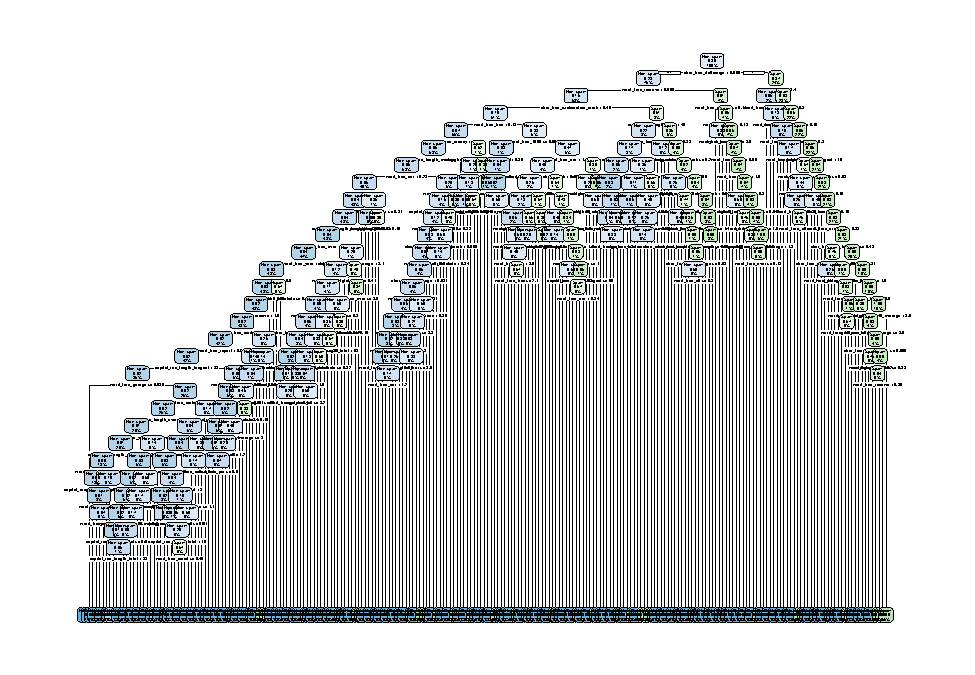
\includegraphics{durand_eltarr_files/figure-latex/unnamed-chunk-23-1.pdf}

Puis élagons cette arbre :

\begin{Shaded}
\begin{Highlighting}[]
\NormalTok{cart.pruned <-}\StringTok{ }\KeywordTok{prune}\NormalTok{(cart}\FloatTok{.0}\NormalTok{, }\DataTypeTok{cp =}\NormalTok{ cart}\FloatTok{.0}\OperatorTok{$}\NormalTok{cptable[}\KeywordTok{which.min}\NormalTok{(cart}\FloatTok{.0}\OperatorTok{$}\NormalTok{cptable[,}\StringTok{"xerror"}\NormalTok{]),}\StringTok{"CP"}\NormalTok{])}
\KeywordTok{rpart.plot}\NormalTok{(cart.pruned)}
\end{Highlighting}
\end{Shaded}

\begin{verbatim}
## Warning: labs do not fit even at cex 0.15, there may be some overplotting
\end{verbatim}

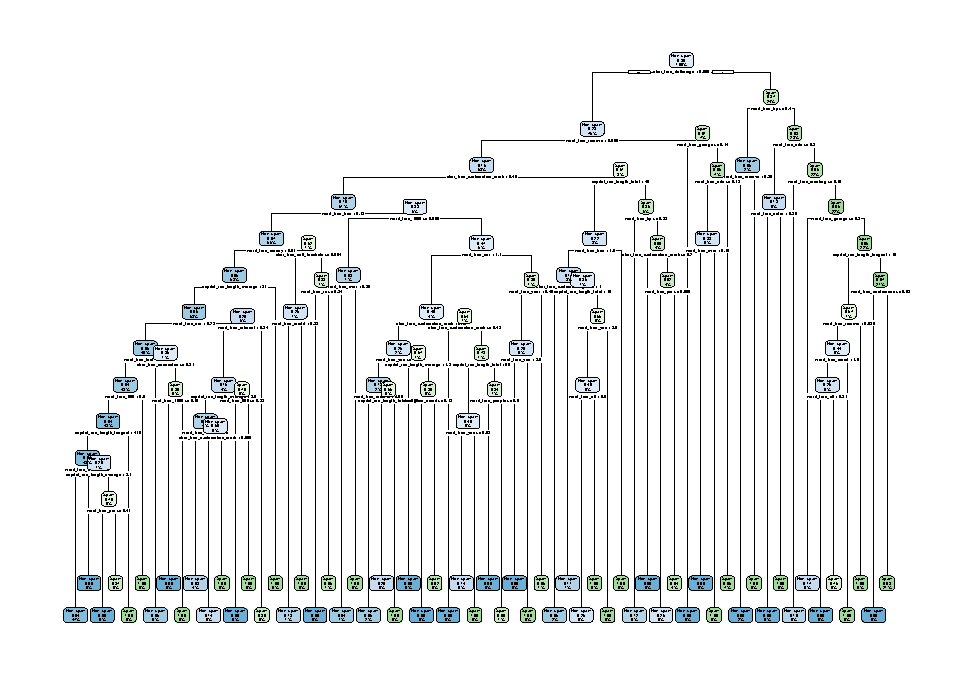
\includegraphics{durand_eltarr_files/figure-latex/unnamed-chunk-24-1.pdf}

Enfin on calcul l'erreur de test (taux de mauvais classement), en
appliquant la règle de Bayes :

\begin{Shaded}
\begin{Highlighting}[]
\NormalTok{pred.pruned <-}\StringTok{ }\KeywordTok{predict}\NormalTok{(cart.pruned, email.te)}
\KeywordTok{mean}\NormalTok{(}\KeywordTok{abs}\NormalTok{(}\KeywordTok{ifelse}\NormalTok{(email.te}\OperatorTok{$}\NormalTok{Class }\OperatorTok{==}\StringTok{ "Spam"}\NormalTok{, }\DecValTok{1}\NormalTok{,}\DecValTok{0}\NormalTok{) }\OperatorTok{-}\StringTok{ }\KeywordTok{ifelse}\NormalTok{(pred.pruned[,}\DecValTok{2}\NormalTok{] }\OperatorTok{>}\NormalTok{.}\DecValTok{5}\NormalTok{, }\DecValTok{1}\NormalTok{,}\DecValTok{0}\NormalTok{)))}
\end{Highlighting}
\end{Shaded}

\begin{verbatim}
## [1] 0.0773913
\end{verbatim}

Nous atteignons donc un taux de mauvais classement de 8\% avec ce
modèle.

Pour

\hypertarget{question-5}{%
\subsection{Question 5}\label{question-5}}

Nous réalisons un bagging 100 arbres de décisions à l'aide de la
fonction bagging de la librairie ipred :

\begin{Shaded}
\begin{Highlighting}[]
\NormalTok{bag.email <-}\StringTok{ }\KeywordTok{bagging}\NormalTok{(Class}\OperatorTok{~}\NormalTok{., }\DataTypeTok{data=}\NormalTok{email.tr, }\DataTypeTok{mfinal=}\DecValTok{100}\NormalTok{)}
\end{Highlighting}
\end{Shaded}

Puis on peut évaluer l'erreur de test :

\begin{Shaded}
\begin{Highlighting}[]
\NormalTok{pred.bag <-}\StringTok{ }\KeywordTok{predict}\NormalTok{(bag.email, email.te)}
\KeywordTok{mean}\NormalTok{(}\KeywordTok{abs}\NormalTok{(}\KeywordTok{ifelse}\NormalTok{(email.te}\OperatorTok{$}\NormalTok{Class }\OperatorTok{==}\StringTok{ "Spam"}\NormalTok{, }\DecValTok{1}\NormalTok{,}\DecValTok{0}\NormalTok{) }\OperatorTok{-}\StringTok{ }\KeywordTok{ifelse}\NormalTok{(pred.bag }\OperatorTok{==}\StringTok{ "Spam"}\NormalTok{, }\DecValTok{1}\NormalTok{,}\DecValTok{0}\NormalTok{)))}
\end{Highlighting}
\end{Shaded}

\begin{verbatim}
## [1] 0.04695652
\end{verbatim}

Nous avons donc une erreur de test de 7,5\%.

\hypertarget{question-6}{%
\subsection{Question 6}\label{question-6}}

Enfin, nous ajustons un modèle random forrest à 100 arbres en choisisant
le mtry, (c'est à dire le nombre de variable que l'on prend pour chaque
arbre), par validation croisée.

\begin{Shaded}
\begin{Highlighting}[]
\NormalTok{cl <-}\StringTok{ }\KeywordTok{makePSOCKcluster}\NormalTok{(}\DecValTok{5}\NormalTok{)}
\KeywordTok{registerDoParallel}\NormalTok{(cl)}

\NormalTok{control <-}\StringTok{ }\KeywordTok{trainControl}\NormalTok{(}\DataTypeTok{method=}\StringTok{"repeatedcv"}\NormalTok{, }\DataTypeTok{number=}\DecValTok{5}\NormalTok{, }\DataTypeTok{repeats=}\DecValTok{10}\NormalTok{)}
\NormalTok{rfGrid <-}\StringTok{  }\KeywordTok{expand.grid}\NormalTok{(}\DataTypeTok{mtry =} \DecValTok{50}\OperatorTok{:}\DecValTok{57}\NormalTok{)}
\NormalTok{RFmodel <-}\StringTok{ }\KeywordTok{train}\NormalTok{(Class}\OperatorTok{~}\NormalTok{., }\DataTypeTok{data=}\NormalTok{email.tr, }\DataTypeTok{method=}\StringTok{"rf"}\NormalTok{, }
                 \DataTypeTok{trControl=}\NormalTok{control,}
                 \DataTypeTok{ntree=}\DecValTok{100}\NormalTok{, }
                 \DataTypeTok{tuneGrid =}\NormalTok{ rfGrid,}
                 \DataTypeTok{verbose=}\OtherTok{FALSE}\NormalTok{)}
\KeywordTok{stopCluster}\NormalTok{(cl)}
\KeywordTok{plot}\NormalTok{(RFmodel)}
\end{Highlighting}
\end{Shaded}

Le choix de mtry est reproductible grâce à la validation croisée.

Puis on peut évaluer l'erreur de test :

\begin{Shaded}
\begin{Highlighting}[]
\NormalTok{pred.rf <-}\StringTok{ }\KeywordTok{predict}\NormalTok{(RFmodel, email.te)}
\KeywordTok{mean}\NormalTok{(}\KeywordTok{abs}\NormalTok{(}\KeywordTok{ifelse}\NormalTok{(email.te}\OperatorTok{$}\NormalTok{Class }\OperatorTok{==}\StringTok{ "Spam"}\NormalTok{, }\DecValTok{1}\NormalTok{,}\DecValTok{0}\NormalTok{) }\OperatorTok{-}\StringTok{ }\KeywordTok{ifelse}\NormalTok{(pred.rf }\OperatorTok{==}\StringTok{ "Spam"}\NormalTok{, }\DecValTok{1}\NormalTok{,}\DecValTok{0}\NormalTok{)))}
\end{Highlighting}
\end{Shaded}

On a une erreur de test de 7\%.

\hypertarget{question-7}{%
\subsection{Question 7}\label{question-7}}

\hypertarget{bootstrap}{%
\section{Bootstrap}\label{bootstrap}}

\hypertarget{question-8}{%
\subsection{Question 8}\label{question-8}}

Ici, on considère une variable aléatoire \(Y\) qui suit une loi normal
de moyenne \(\theta\) et de variance 1. On souhaiterait estimer son
espérance par estimateur du maximul de vraisemblance.

\begin{Shaded}
\begin{Highlighting}[]
\NormalTok{y =}\StringTok{ }\KeywordTok{rnorm}\NormalTok{(}\DecValTok{100}\NormalTok{,}\DecValTok{4}\NormalTok{,}\DecValTok{1}\NormalTok{)}
\end{Highlighting}
\end{Shaded}

On a pour la vraisemblance \begin{align*}
L(y_1,\dots,y_n\mid \theta) &= \displaystyle \prod_{i=1}^n \farc{1}{sqrt{2\pi}}e^{(y_i-\theta)^2/2}\\
&= \displaystyle \farc{1}{sqrt{2\pi}^n}e^{\sum_{i=1}^n(y_i-\theta)^2/2}\\
\mbox{En passant au log}\\
\implies\\
log(L(y_1,\dots,y_n\mid \theta)) &= \displaystyle log(\farc{1}{sqrt{2\pi}^n})  + \sum_{i=1}^n(y_i-\theta)^2/2
\end{align*} Maximisier la vraisemblance revient à maximiser
\(\displaystyle \frac{1}{2}\sum_{i=1}^n(y_i-\theta)^2\). On en déduit
que l'EMV ici est
\[\displaystyle \hat{\theta} = \frac{1}{n}\sum_{i=1}^ny_i.\] Il coïncide
avec l'estimateur des moments et avec la moyenne empirique. On va
produire plusieurs valeurs de \(\hat{\theta}\) :

\begin{Shaded}
\begin{Highlighting}[]
\NormalTok{n <-}\StringTok{ }\DecValTok{100}
\NormalTok{N <-}\StringTok{ }\DecValTok{1000}
\KeywordTok{set.seed}\NormalTok{(}\DecValTok{11}\NormalTok{)}
\NormalTok{theta_hat <-}\StringTok{ }\KeywordTok{rowMeans}\NormalTok{(}\KeywordTok{matrix}\NormalTok{(}\KeywordTok{rnorm}\NormalTok{(N}\OperatorTok{*}\NormalTok{n,}\DecValTok{2}\NormalTok{,}\DecValTok{1}\NormalTok{), N,n))}
\KeywordTok{boxplot}\NormalTok{(theta_hat,}\DataTypeTok{col =} \StringTok{'darkseagreen3'}\NormalTok{)}
\end{Highlighting}
\end{Shaded}

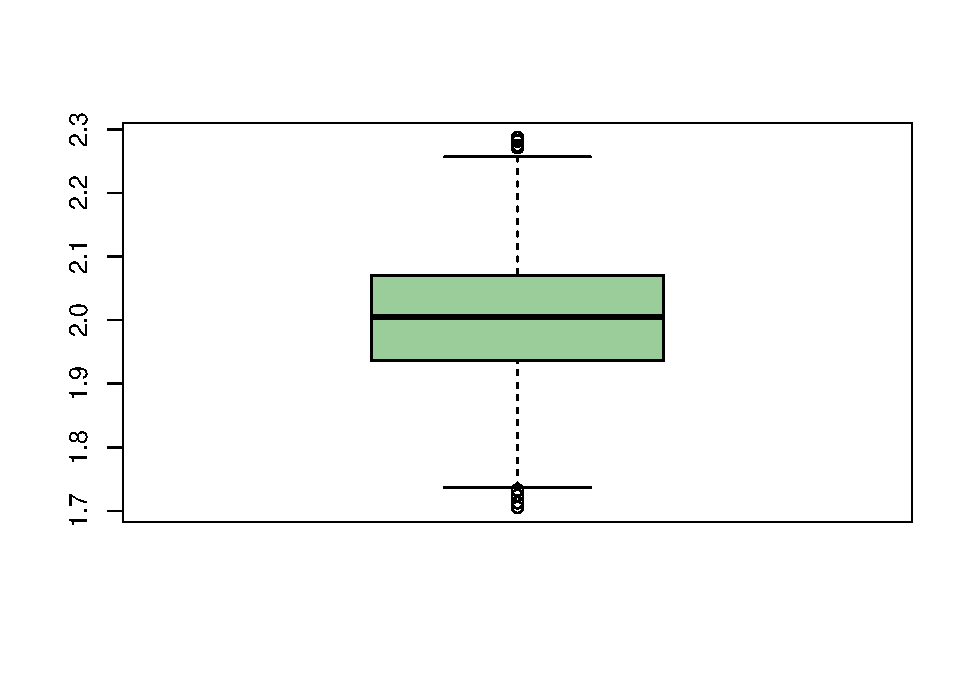
\includegraphics{durand_eltarr_files/figure-latex/unnamed-chunk-31-1.pdf}

\begin{Shaded}
\begin{Highlighting}[]
\KeywordTok{hist}\NormalTok{(theta_hat, }\DataTypeTok{ylab=}\StringTok{"Fréquence"}\NormalTok{, }\DataTypeTok{xlab=}\StringTok{"Estimateur"}\NormalTok{,}\DataTypeTok{main=}\StringTok{"Histograme de l'estimateur"}\NormalTok{, }\DataTypeTok{col=}\StringTok{"orange"}\NormalTok{,}\DataTypeTok{breaks =} \DecValTok{40}\NormalTok{)}
\NormalTok{xx <-}\KeywordTok{seq}\NormalTok{(}\FloatTok{1.6}\NormalTok{, }\FloatTok{2.4}\NormalTok{, }\DataTypeTok{le=}\DecValTok{200}\NormalTok{)}
\NormalTok{et <-}\StringTok{ }\DecValTok{1}\OperatorTok{/}\KeywordTok{sqrt}\NormalTok{(n)}
\KeywordTok{points}\NormalTok{(xx,}\KeywordTok{dnorm}\NormalTok{(xx, }\DecValTok{4}\NormalTok{, et), }\DataTypeTok{type=}\StringTok{"l"}\NormalTok{, }\DataTypeTok{lwd =} \DecValTok{2}\NormalTok{, }\DataTypeTok{col=}\StringTok{"red"}\NormalTok{)}
\end{Highlighting}
\end{Shaded}

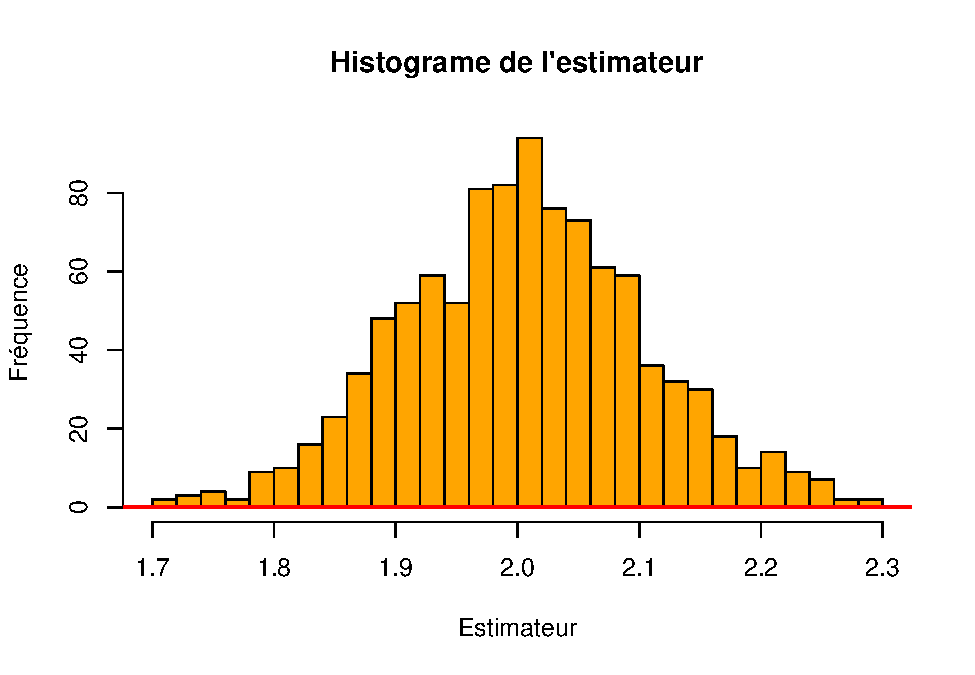
\includegraphics{durand_eltarr_files/figure-latex/unnamed-chunk-31-2.pdf}

\hypertarget{autour-de-lalgorithme-adaboost}{%
\section{Autour de l'algorithme
Adaboost}\label{autour-de-lalgorithme-adaboost}}

\hypertarget{question-10}{%
\subsection{Question 10}\label{question-10}}

\begin{tabular}{|l|c|c|c|r|} \hline & &  \textbf{Perte}  & &  \\ & & \textbf{exponentielle} & \textbf{Perte binaire} & \\ $\hat{c}(x_*)$ & $\hat{y}_*$ & $exp(-y_* \hat{c}(x_*))$ &   $1(y_* \neq \hat{y}_*)$ & $y_*$ \tabularnewline \hline 0.3 & & & & -1 \tabularnewline \hline -0.2 & & & & -1 \tabularnewline \hline 1.5 & & & & 1 \tabularnewline \hline -4.3 & & & & 1 \tabularnewline \hline \end{tabular}

\end{document}
